\section{Examples}\label{sec:examples}

The sections above illustrate each part of the code on its own. Here I
give two examples that combine several of them in a single analysis, of
the kind that the backends were built for. Both are deliberately small:
they use mock data and run in minutes, and their point is the shape of
the computation rather than the result.

\subsection{A hypervelocity star as a probe of the potential}\label{sec:examples-hvs}

A hypervelocity star ejected from the Galactic center must, when its
orbit is integrated backwards, return to the Galactic center, and the
closest approach of the backward orbit to the center is therefore a
function of the Galactic potential that a measurement of the star's
phase-space position constrains \citep[see, \eg,][]{Gnedin2005,Contigiani2019}.
This is a natural problem for differentiable orbits, because the
objective---the distance of closest approach---is a function of an
integrated orbit, and both the star's initial condition, within its
uncertainties, and the potential's parameters are to be varied.
\figurename~\ref{fig:hvs} displays the two derivatives of
\sectionname~\ref{sec:orbit-paths} at work on a mock star resembling
S5-HVS1 in a cored, flattened logarithmic halo. In the left panel the
potential is held fixed and the star's phase-space position is adjusted
within its observational uncertainties to minimize the closest approach,
using the derivative of the orbit with respect to its initial condition
from the \cc\ variational integrator; seven Gauss--Newton iterations
bring the closest approach from $0.2$ to $0.1$\,kpc. In the right panel
the star is held fixed and the flattening $q$ of the halo is fit by
descending the closest approach with the derivative obtained by
reverse-mode differentiation through the in-backend orbit integration,
which the \cc\ path cannot provide; the recovered $q=0.851$ matches the
true $0.85$ from which the mock star was generated. In code, the second
fit is
\begin{code}
def closest_approach(q):
    pot= LogarithmicHaloPotential(normalize=1.,core=0.2,q=q)
    o= Orbit(jnp.asarray(vxvv),radec=True,ro=8.,vo=220.)
    o.integrate(-ts,pot,method='diffrax')
    return jnp.min(o.r(-ts))
objective= jax.jit(jax.value_and_grad(closest_approach))
q= adam_descent(objective,q0=1.1) # a few lines of optax
\end{code}
With real
data, the two fits would be combined into one likelihood over the star's
parameters and those of the potential, and the derivative of that
likelihood with respect to all of them would be available for a
gradient-based sampler.

\begin{figure*}[t!]
  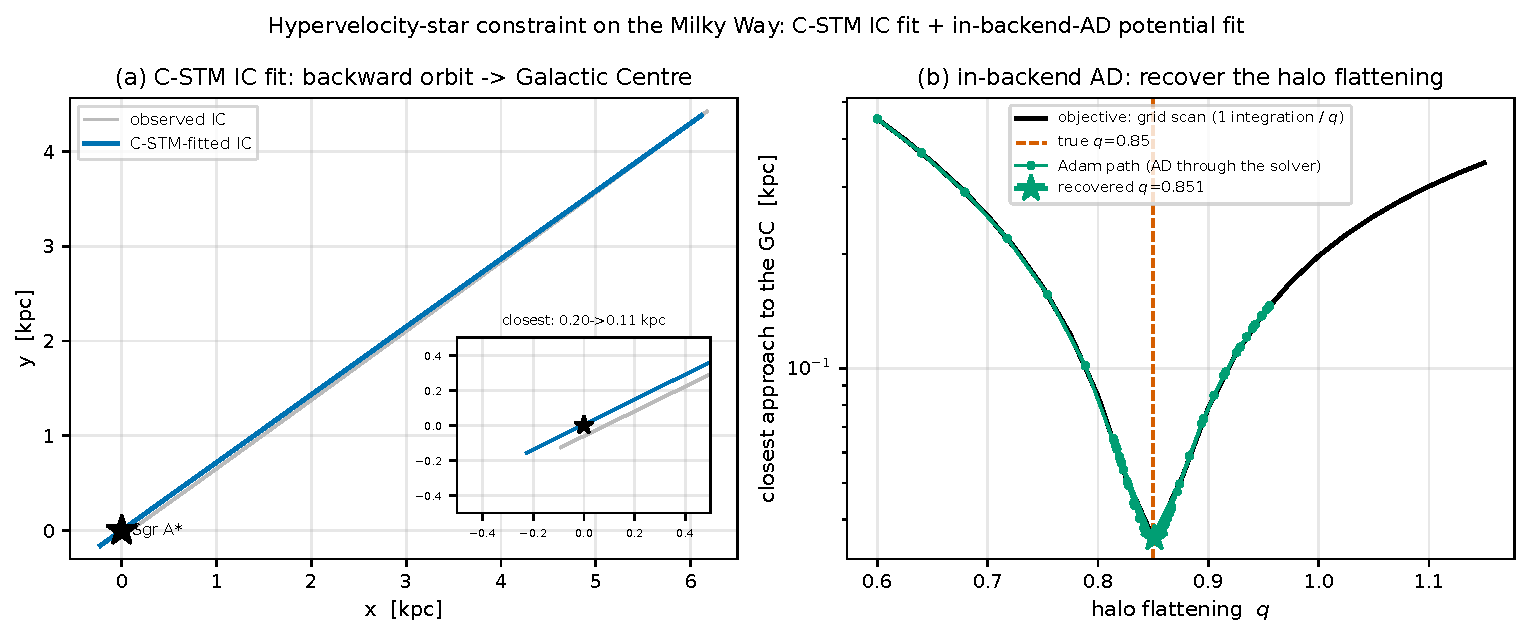
\includegraphics[width=\textwidth,clip=]{../figures/g14_hvs_potential_fit/g14_hvs_potential_fit.pdf}
  \caption{A mock hypervelocity star as a constraint on the Galactic potential.
    Left: the orbit of a star resembling S5-HVS1, integrated backwards
    from its observed phase-space position (grey) and from the position
    within the observational uncertainties that brings the orbit closest
    to Sgr~A$^*$ (blue), found by Gauss--Newton iterations on the
    derivative of the orbit with respect to its initial condition from
    the \cc\ variational integrator. Right: the closest approach to the
    Galactic center of the backward orbit as a function of the
    flattening $q$ of the halo (black, from a grid of integrations) and
    the path of a gradient-descent fit of $q$ using the derivative of the
    closest approach through the in-backend orbit integration (points),
    which recovers the value from which the star was generated (dashed
    line).}\label{fig:hvs}
\end{figure*}

\subsection{Learning the inverse action--angle transformation}\label{sec:examples-neural}

The transformation from actions and angles to positions and velocities
has no closed form in a general potential, and \galpy's implementations
of it are limited to one-dimensional potentials and to the torus
machinery. A differentiable forward transformation makes a different
approach possible: a neural network $G(\vecj,\veca)$ that takes actions
and angles to phase-space positions can be trained by requiring that
\galpy's forward transformation, applied to the network's output,
return the actions and angles that went in. The loss is then a cycle
consistency, $|F(G(\vecj,\veca))-(\vecj,\veca)|^2$, with $F$ the
\texttt{actionAngle} method, and its gradient with respect to the
network's weights flows through $F$. No reference inverse is needed
anywhere in the training. \figurename~\ref{fig:neural} shows this for
the vertical motion in \texttt{MWPotential2014} at the solar radius,
where the exact inverse of \sectionname~\ref{sec:aa-other} exists and
serves as a check, and for the full axisymmetric case with the
St\"{a}ckel approximation, where no reference exists. In the first case a
small network trained in a few minutes, identically under \jax\ and
\torch, reproduces the exact tori to a phase-space error of $0.5$ to
$2\,\%$; in the second, a four-layer network trained for half an hour on
a GPU returns actions on the round trip with a scatter of $7\times10^{-3}$
and reconstructs the meridional orbits that it has never seen. Neither
network is a replacement for a proper inverse, and the point is not the
accuracy of these particular fits but that \galpy's action--angle code
sits inside a training loop, as a layer whose gradient the framework
computes, and that the same code does so in both frameworks.

\begin{figure*}[t!]
  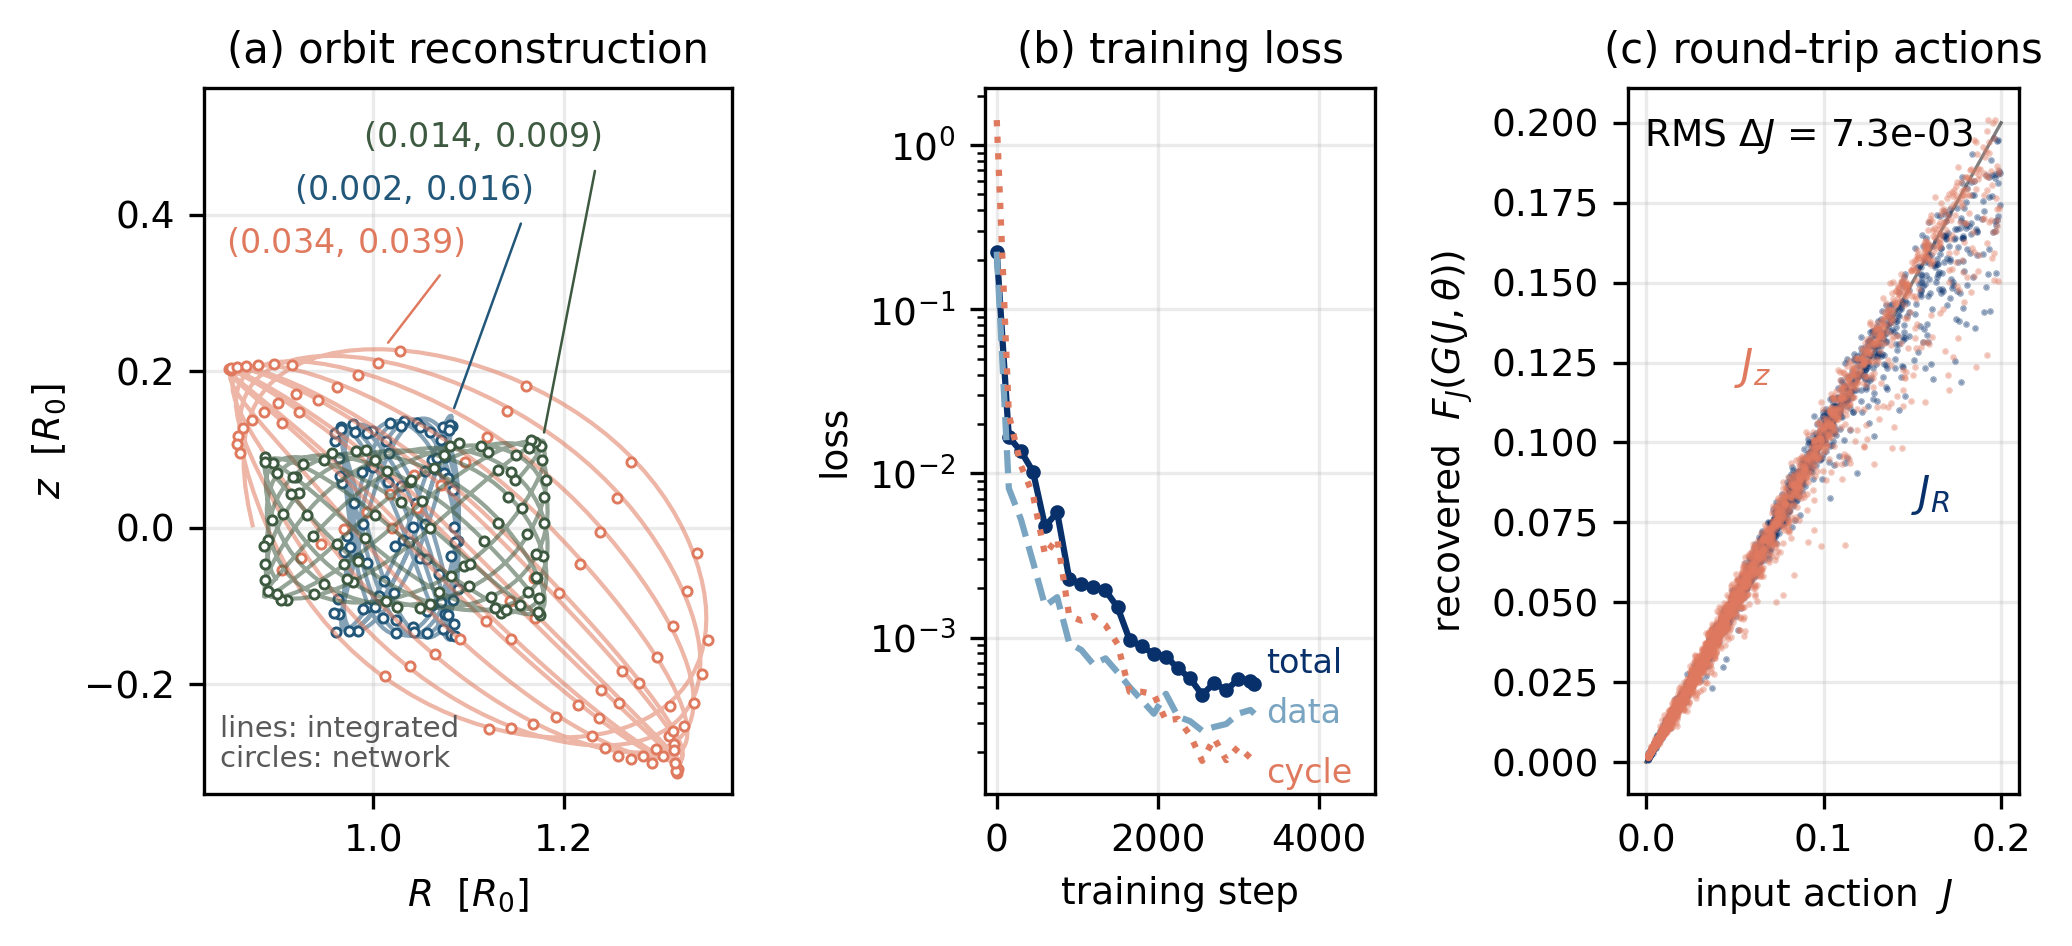
\includegraphics[width=\textwidth,clip=]{../figures/g20_neural_staeckel_inverse/g20_neural_staeckel_inverse.png}
  \caption{Neural inverse of the St\"{a}ckel action--angle transformation
    in \texttt{MWPotential2014} at fixed $L_z$, learned by differentiating
    through \galpy's forward transformation.
    Left: three orbits integrated in the potential (lines) and the
    positions returned by the network for the orbits' actions and
    angles (circles). Middle: the training loss, with its data and
    cycle-consistency terms. Right: the actions recovered by applying
    the forward transformation to the network's output against the
    input actions for a test set.}\label{fig:neural}
\end{figure*}
